\section{Introducción}
Esta sección se enfocará a la parte de transmisión de información y que tipo de operaciones lógicas matemáticas ocurren para que un cerebro pueda realizar cómputos, específicamente se detallará la mecánica de los disparos de las neuronas, siendo estos una de las características más relevantes a la hora de modelar las redes neuronales artificiales. Si en algún momento de su vida han visto temas relacionados con compuertas digitales, arquitectura de computadoras, diseño electrónico digital, les será más fácil abstraer el concepto, pues nosotros vamos a ver los procesos de paso de información a través de compuertas pero en un sistema biológico (de la naturaleza). 

Notemos primeramente un impulso nervioso, recordemos que esté es una onda que avanza desde el cono axónico de la neurona hasta la neurona postsináptica. Esta onda electroquímica ocurre dada la diferencia de potencial entre la parte interna y externa de neurona, está diferencia se da a consecuencia de las distintas concentraciones de iones en ambos lados de la membrana plasmática. Los estados en la membrana plasmática (del axón) se pueden diferenciar en, potenciales neuronales:

\begin{itemize}
\item \textbf{Potencial de reposo:} Es la diferencia de cargas en la membrana y está polarizada a -70mV. Es positiva por fuera (Na+ ) y negativa por dentro por Cl- y proteínas- y no transmite señal. 
\item \textbf{Potencial de acción o membrana:} Un estímulo umbral de 55mV, despolariza la membrana y abre los canales del Na+ y K+ y avanza la señal nerviosa, es un cambio muy rápido en la polaridad de la membrana de negativo a positivo y vuelta a negativo.
\end{itemize}

%(Insertar esquema) 
\begin{figure}[h]
 \centering
 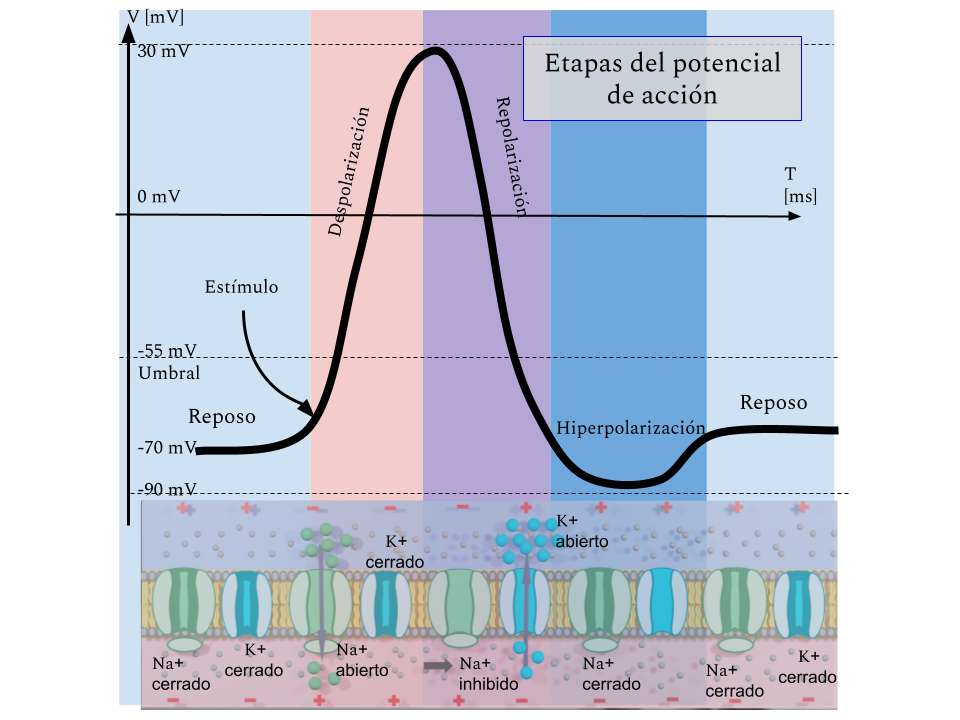
\includegraphics[scale=0.5]{../Figuras/Grafica.png}
 \caption{Representación gráfica de la respuesta de los canales ionicos de sódio (Na+ en verde) y potasio (K+ en azul) ante un estímulo de voltaje, dando como resultado un potencial de acción que viajará a lo largo de todo el axón.}
 \label{fig:graficaP}
\end{figure}

Retomando la sinapsis eléctrica, donde participan los canales iónicos y las entradas de la neuronas (dendritas) están siendo alteradas poco a poco, hasta que ocurre la suficiente carga (diferencia de potencial) en sus dendritas y en el cuerpo de la neurona, para que desde el cono axónico se de un disparo o potencial de acción (spike), transmitiendo la información gracias a la apertura y cierre de ciertos canales de iones cargados. Este cambio brusco de la diferencia de potencial, se nota en forma de un pulso eléctrico (ver \ref{fig:graficaP}),  para saber más a detalle qué está ocurriendo en está rápida elevación en la diferencia de potencial, se contará de dónde salió este modelo y por qué toma la forma que tiene. 

Los primeros científicos que estudiaron el potencial de acción y dieron un modelo (de la unión sináptica eléctrica) fueron Alan Lloyd Hodgkin y Andrew Fielding Huxley alrededor de 1952, obteniendo un modelo matemático, que intenta explicar qué es lo que estaba pasando en las neuronas. Ellos trabajaron con un calamar gigante (que puede medir hasta 4 metros de largo) que dado su gran tamaño, tiene un axón también bastante gigantesco, que recorre casi la mitad del cuerpo del calamar y su grosor es de medio milímetro, considerando el tamaño estándar de una axón de una neurona (1-20 µm). El axón del calamar gigante es tan grande que les permitió introducir dispositivos para medir el voltaje, es decir, la diferencia de potencial entre, el interior de la neurona y la parte de afuera (el ambiente externo de la neurona). Con estás mediciones experimentales que lograron obtener (1939), se pudo determinar qué pasaba con las cargas eléctricas tanto en el interior como en el exterior y así estudiar cómo se lograba la transferencia de electricidad cuando disparaba este pulso. 
 Se dan cuenta que podían modelar este comportamiento como un circuito eléctrico donde están corriendo estas corrientes, si bien aún no sabían todavía cuál era exactamente el mecanismo biológico por detrás, si observaron que había dos elementos protagónicos que serían el sodio y el potasio.
 Notaron que estos existen en diferentes concentraciones, en la parte de afuera y en la parte de adentro de las neuronas. Con esto nosotros podemos aprender también el por qué es importante consumir algo de sal y nunca estar bajos de potasio, pues estos dos elementos son indispensables para que las neuronas puedan transmitir sus señales. 

\section{Membrana y canal}

Hodgkin y Huxley se dedicaron a estudiar qué pasaba con las concentraciones de estos iones (sodio y potasio) en la parte de afuera o en la parte de adentro cuando empezaban a fluir las corrientes. El sistema parecía una especie de circuito eléctrico, se lo imaginaron como una especie de membrana porosa (lo cual es bastante cercano a lo que después se descubrió  con la microscopía) y la forma en que lo vieron fue como un circuito eléctrico donde  \textit{la membrana está funcionando como un capacitor} que almacena ligeramente las cargas cuando están tratando de pasar de un lado hacia el otro y además con la cualidad que tenía de veces dejar pasar más iones y a veces no (semipermeable), modelan esto como una especie de \textit{resistencias variables}. Bajo ciertas condiciones de voltaje de la diferencia de potencial entre la parte de afuera y la parte de adentro, estos canales permiten pasar más de estos iones (ya sean sodio, potasio o calcio) o por el contrario impiden su paso (ver \ref{fig:ModelHh}).


\begin{figure}[h]
 \centering
 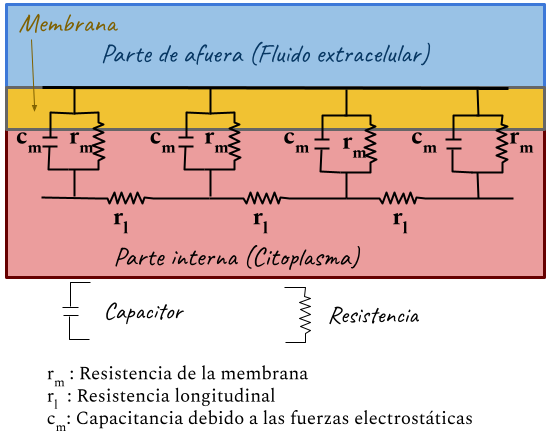
\includegraphics[scale=0.5]{../Figuras/ModeloHH.2}
 \caption{Un primer modelo de la membrana axónica modelada como circuito eléctrico. La parte amarilla es la membrana}
 \label{fig:ModelHh}
\end{figure}


Ahora se necesitan más detalles de la representación de los canales y toman en cuenta que el comportamiento de estas resistencias viene acompañado con un voltaje de reposo, en estos voltajes particulares cada tipo de ion (de la resistencia modelada) se estabiliza y ya no va a cambiar esta resistencia (ver \ref{fig:circuito}). 


\begin{figure}[h]
 \centering
 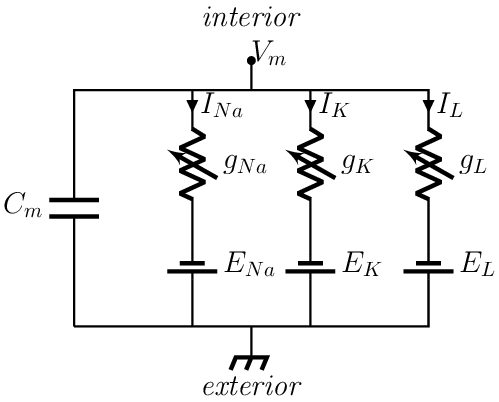
\includegraphics[scale=0.5]{../Figuras/circuito.png}
 \caption{Modelo de la membrana axónica modelada como circuito eléctrico, con los distintos canales presentes y su voltaje de reposo.}
 \label{fig:circuito}
\end{figure}

Lo que observan es que el \textbf{ion de sodio (Na+)} y su resistencia va a variar dependiendo del voltaje, a esto se le llama un \textbf{canal transitorio} porque en ciertos voltajes si puede pasar; si es muy bajo, no puede pasar y si rebasa un cierto umbral entonces se vuelve a tapar y ya no puede pasar. 
Lo que sucede con el \textbf{ion de potasio (K+)} es que, puede salir si el voltaje está más allá de un cierto valor, si no, no pasan y va variando un poquito que tanto puede pasar, a esto se le llama \textbf{canal persistente}. Por estas características de que el potasio es un intervalo dentro de la recta y el sodio es a partir de cierto valor, por tanto se les modelan de maneras ligeramente diferentes. Más adelante se descubrió porque tenían este comportamiento, básicamente el canal de potasio es una puerta hecha de cuatro subpuertas por donde los elementos pasan o no pasan, el canal de sodio es como una compuerta que está hecha de tres subpuertas que se pueden abrir y tiene aparte un tapón extra, que hace que  aunque estas tres están abiertas bloquee toda la compuerta.
Las neuronas están trabajando con muchos más iones aparte de estos dos, uno que destaca bastante es el caso del cloro (Cl-) que tiene carga negativa. Se tienen canales para intercambio aleatorio de otros iones, L Un canal aleatorio (leaky).

Entonces con lo que ellos midieron experimentalmente, midieron cómo se estaban comportando estas resistencias dependiendo del voltaje o la diferencia de potencial que había entre ambos lados de la membrana y a partir de ahí pudieron describir matemáticamente y simular los disparos que se conocen como potenciales de acción vamos a ver cuáles fueron estos conceptos de electricidad que se están utilizando para el modelo tenemos este concepto de potenciales eléctricos.

\begin{itemize}
\item Potenciales eléctricos \emph{E ó  V}; resultan de la separación de cargas opuestas. Se mide en \emph{mV}.
\item Corriente \emph{I}; Movimiento de cargas. Se mide en \emph{µA}.
\item Resistencia \emph{R}; Medida de la oposición al movimiento de las partículas cargadas.
\item Conductancia \emph{g}; Inverso de la resistencia (1/r), es decir, facilidad de transmisión de las partículas cargadas.
\item Capacitancia o capacidad eléctrica \emph{C} . Cantidad de energía eléctrica almacenada en un capacitor para una diferencia de potencial eléctrico dada.
\end{itemize}

Lo que está pasando en los potenciales eléctricos es que hay mucho sodio en la parte externa de la membrana por ej. tres iones de sodio que son cargas positiva por dos iones de potasio que hay en la parte interna, entonces hay muchas más cargas positivas en la parte de afuera que las que hay en la parte de adentro y eso es lo que provoca  la diferencia de cargas que es lo que estamos viendo como un  potencial eléctrico.

Durante el experimento con el axón, se le dierón cargas electricas directamente al axón y gracias a eso lograban ir midiendo que era lo
que estaba pasando con las concentraciones de cargas afuera y adentro en el caso de las neuronas reales, esto en un ambiente no alterado ocurre cuando entran en juego los neurotransmisores y provocan que haya cambios, precisamente en estas corrientes. Entonces hodgkin y huxley  jugaron el rol que tendrían que jugar usualmente los neurotransmisores para abrir otras compuertas. Nosotros en la manera en la que lo vamos a simular es precisamente con estas corrientes que son las que se están poniendo en el experimento y vamos a ver cómo reacciona el axón. 

La  capacidad eléctrica o capacitancia es la que estamos utilizando para modelar la membrana conformada por lípidos, que es una  capa de grasa y esa es la cantidad de energía eléctrica almacenada en un capacitor para una diferencia de potencial eléctrico dada y éste tiene un comportamiento bastante interesante porque las cargas quedan almacenadas un momento pero se van liberando poco a poco y se va descargando ese capacitor. 

\section{Potenciales de Nerst o de reposo}

Son los potenciales a los cuales el flujo neto de iones a través de los canales abiertos es cero.
Aquí vemos precisamente porque estamos utilizando la \emph{E} generalmente la vamos a utilizar para referirnos a la diferencia de potencial entre la parte de afuera de la célula y la parte de adentro  las vamos a utilizar para representar a aquellos voltajes donde cada una de las compuertas encontrarían su equilibrio . Esos voltajes son distintos para cada una de las compuertas, esto va a provocar precisamente la dinámica de la de la neurona, por ejemplo: 

\begin{itemize}
\item E \textsubscript{Na}  \emph{50mV}
\item E \textsubscript{Ca}  \emph{150mV}
\item E \textsubscript{K}   \emph{− 80mV}
\item E \textsubscript{Cl}  \emph{− 60mV}
\end{itemize}

Aquí vemos que el sodio estaría su equilibrio en un valor positivo, 
el calcio que es el que va a jugar un rol de que se activen los neurotransmisores y se transmita el disparo, observamos que el voltaje tendría que ser bastante positivo. El potasio que es el que usualmente está trabajando intercambiándose casi todo el tiempo en la neurona, veremos que el punto de equilibrio usual de la neurona anda por los -76mV y el del cloro, cada uno de estos canales pues está tratando de jalar la dinámica hacia su potencial de equilibrio y no hay precisamente un acuerdo entre ellos y eso es precisamente lo que hace que las neuronas cobren "vida".

\section{Modelo de la membrana como bicapa de lípidos}
La membrana de una neurona es modelada como un elemento de un circuito con capacitancia \emph{C\textsubscript{m}} y potencial \emph{V} , los cuales están regidos por las ecuaciones siguientes:


\section{Modelo de las compuertas iónicas controladas por voltaje}
\section{Dinámica del voltaje durante un disparo} 
\section{Simulación usando el método de Euler}
\section{Información condificada en las dendritas}

